\documentclass[12pt, letterpaper]{article}
\usepackage{graphicx} % Required for inserting images
\usepackage{hyperref}
\usepackage{listings}
\usepackage{amssymb}
\usepackage{amsmath}
\usepackage[english]{babel}
\usepackage{nicefrac, xfrac}
\usepackage{mathtools}
\newcommand{\acc}{\\\hphantom{}\\}
\usepackage[table,xcdraw]{xcolor}
\usepackage[paper=a4paper,left=20mm,right=20mm,bottom=25mm,top=25mm]{geometry}
\renewcommand{\labelenumii}{\arabic{enumi}.\arabic{enumii}}
    \renewcommand{\labelenumiii}{\arabic{enumi}.\arabic{enumii}.\arabic{enumiii}}
    \renewcommand{\labelenumiv}{\arabic{enumi}.\arabic{enumii}.\arabic{enumiii}.\arabic{enumiv}}
\title{Voli aerei 2 (gruppo 42)}
% \author{ Giacomo Biribicchi \and Marco Casu \and Christian Di Manno \and Alessandro Gautieri }
\date{}


\begin{document}

\maketitle


\section{Requisiti}

I dati di interesse per il sistema sono \underline{Voli}, \underline{Compagnia} ed \underline{Aeroporti}.
\begin{enumerate}
    \item \textbf{Volo}\begin{enumerate}
        \item codice - Serie di caratteri alfanumerici che identificano univocamente un \underline{Volo}.
        \item durata - Si usa un dato composto, consistente in un intero positivo per identificare la durata in ore, e due interi 
        compresi fra 0 e 59, rispettivamente per i minuti ed i secondi.
        \item compagnia - La compagnia che fornisce il volo.
        \item aereoporto di partenza 
        \item aereoporto di arrivo
        \item VoloCharter - Sarà una sottoclasse di Volo, permetterà di modellare i voli di tipo charter con le 
        relative tappe intermedie.
    \end{enumerate}
    \item \textbf{Aereoporto}\begin{enumerate}
        \item codice - Serie di caratteri alfanumerici che identificano univocamente un \underline{Aereoporto}.
        \item nome 
        \item città - La città in cui risiede l'\underline{Aereoporto}.
        \item nazione - La nazione in cui si trova la città.
    \end{enumerate}
    \item \textbf{Compagnia}\begin{enumerate}
        \item nome 
        \item anno di fondazione 
        \item città sede direzione
    \end{enumerate}
    \item \textbf{TappaIntermedia}\begin{enumerate}
        \item ordine - L'ordine della tappa all'interno di un volo charter.
    \end{enumerate}
    \item \textbf{Veivolo}\begin{enumerate}
        \item nome modello 
        \item capienza
    \end{enumerate}
\end{enumerate}
Saranno necessarie due classi \underline{Città} e \underline{Nazione}.\newpage
\section{Considerazioni}
Un \underline{Volo} può appartenere a più di una \underline{Compagnia}? No.\acc 
Un \underline{Volo} può cambiare \underline{Compagnia}? Se si, si vuole mantenere uno storico? No, non si vuole far si che uno stesso 
\underline{Volo} possa cambiare compagnia mantenendo lo stesso codice, sarà semplicemente un altro  \underline{Volo}, con codice 
diverso e \underline{Compagnia} diversa, ma con il tragitto e durata identici.\acc
I Voli di tipo charter hanno sempre una partenza ed un arrivo, la loro relazione con le \underline{TappeIntermedie} non 
fa riferimento a questi due, ma esclusivamente agli aereoporti di "scalo".
\acc 
Ogni \underline{VoloCharter} ha associati più modelli di \underline{Veivolo}, un modello per ogni tappa.
\acc 
Ogni \underline{TappaIntermedia}, che ha ordine $x$, ha associato un modello di veivolo, esso fa riferminto all'aereo utilizzato 
per la tratta $x-1$-$x$.\acc 
I \underline{Veivoli} non hanno un codice identificativo, perché non ci interessa rappresentare il singolo 
\underline{Veivolo} associato ad una tappa, ma il suo modello.
\section{UML}
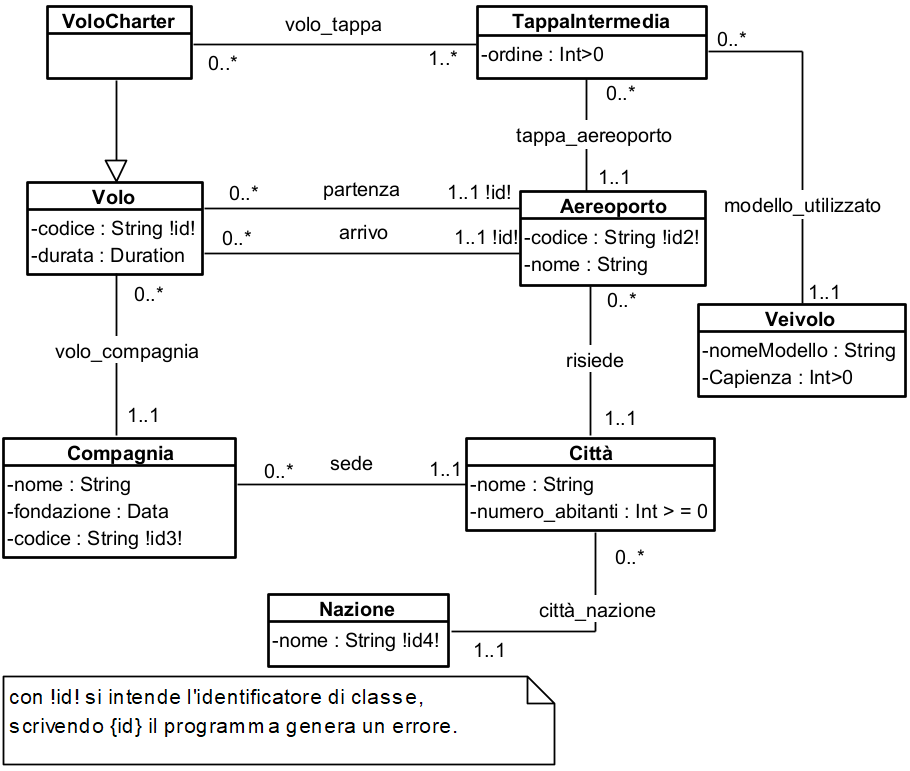
\includegraphics[width=\textwidth]{images/UML.png}


\end{document}

